%% V1.3
%% 2007/01/11
%% by Michael Shell
%% see http://www.michaelshell.org/
%% for current contact information.
%%
%% This is a skeleton file demonstrating the use of IEEEtran.cls
%% (requires IEEEtran.cls version 1.7 or later) with an IEEE journal paper.
%%
%% Support sites:
%% http://www.michaelshell.org/tex/ieeetran/
%% http://www.ctan.org/tex-archive/macros/latex/contrib/IEEEtran/
%% and
%% http://www.ieee.org/



% *** Authors should verify (and, if needed, correct) their LaTeX system  ***
% *** with the testflow diagnostic prior to trusting their LaTeX platform ***
% *** with production work. IEEE's font choices can trigger bugs that do  ***
% *** not appear when using other class files.                            ***
% The testflow support page is at:
% http://www.michaelshell.org/tex/testflow/


%%*************************************************************************
%% Legal Notice:
%% This code is offered as-is without any warranty either expressed or
%% implied; without even the implied warranty of MERCHANTABILITY or
%% FITNESS FOR A PARTICULAR PURPOSE! 
%% User assumes all risk.
%% In no event shall IEEE or any contributor to this code be liable for
%% any damages or losses, including, but not limited to, incidental,
%% consequential, or any other damages, resulting from the use or misuse
%% of any information contained here.
%%
%% All comments are the opinions of their respective authors and are not
%% necessarily endorsed by the IEEE.
%%
%% This work is distributed under the LaTeX Project Public License (LPPL)
%% ( http://www.latex-project.org/ ) version 1.3, and may be freely used,
%% distributed and modified. A copy of the LPPL, version 1.3, is included
%% in the base LaTeX documentation of all distributions of LaTeX released
%% 2003/12/01 or later.
%% Retain all contribution notices and credits.
%% ** Modified files should be clearly indicated as such, including  **
%% ** renaming them and changing author support contact information. **
%%
%% File list of work: IEEEtran.cls, IEEEtran_HOWTO.pdf, bare_adv.tex,
%%                    bare_conf.tex, bare_jrnl.tex, bare_jrnl_compsoc.tex
%%*************************************************************************

% Note that the a4paper option is mainly intended so that authors in
% countries using A4 can easily print to A4 and see how their papers will
% look in print - the typesetting of the document will not typically be
% affected with changes in paper size (but the bottom and side margins will).
% Use the testflow package mentioned above to verify correct handling of
% both paper sizes by the user's LaTeX system.
%
% Also note that the "draftcls" or "draftclsnofoot", not "draft", option
% should be used if it is desired that the figures are to be displayed in
% draft mode.
%
\documentclass[journal, ]{IEEEtran}
\usepackage{cite}
\usepackage[pdftex]{graphicx}
\usepackage[cmex10]{amsmath}
% Also, note that the amsmath package sets \interdisplaylinepenalty to 10000
% thus preventing page breaks from occurring within multiline equations. Use:
%\interdisplaylinepenalty=2500
\usepackage{algorithmic}
\usepackage{array}
\usepackage{mdwmath}
\usepackage{mdwtab}
\usepackage{eqparbox}
%\usepackage[tight,footnotesize]{subfigure}
%\usepackage[caption=false]{caption}
\usepackage[font=footnotesize]{subfig}
\usepackage{fixltx2e}
\usepackage{stfloats}

\ifCLASSOPTIONcaptionsoff
  \usepackage[nomarkers]{endfloat}
  \let\MYoriglatexcaption\caption
  \renewcommand{\caption}[2][\relax]{\MYoriglatexcaption[#2]{#2}}
\fi
\usepackage{url}

% *** Do not adjust lengths that control margins, column widths, etc. ***
% *** Do not use packages that alter fonts (such as pslatex).         ***

% correct bad hyphenation here
\hyphenation{op-tical net-works semi-conduc-tor}

\begin{document}
\title{Real or Not? NLP with Disaster Tweets EDA}

% author names and IEEE memberships
% note positions of commas and nonbreaking spaces ( ~ ) LaTeX will not break
% a structure at a ~ so this keeps an author's name from being broken across
% two lines.
% use \thanks{} to gain access to the first footnote area
% a separate \thanks must be used for each paragraph as LaTeX2e's \thanks
% was not built to handle multiple paragraphs
\author{Vegar~Andreas~Bergum,~\IEEEmembership{vab1g19,}
        ChanKai~Fu,~\IEEEmembership{ckf1n19,}
        Adam~Ghoumrassi,~\IEEEmembership{ag3u19,}
        and~PingChun~Tsai,~\IEEEmembership{pct1g19.}% <-this % stops a space
 }
% \author{....lastname \thanks{...} \thanks{...} }
%                     ^------------^------------^----Do not want these spaces!

% The paper headers
\markboth{COMP6208 Advanced Machine Learning}
{}
% The only time the second header will appear is for the odd numbered pages
% after the title page when using the twoside option.
% you desire.

\maketitle

\begin{abstract}
Lorem ipsum dolor sit amet, consectetur adipiscing elit. Fusce eget erat mi.
Nam non diam felis. Ut tincidunt, mauris eget ornare sodales, orci ligula
bibendum dui, id tristique augue arcu eu dolor. Vestibulum tortor justo,
malesuada at ligula eget, cursus laoreet diam. Orci varius natoque penatibus et
magnis dis parturient montes, nascetur ridiculus mus. Ut non volutpat metus, id
luctus nunc. Duis nisi nunc, ullamcorper at enim at, maximus luctus sem.
Quisque ipsum risus, tempor nec sem vitae, placerat placerat tellus. Nunc
congue, diam facilisis eleifend elementum, sapien sem viverra risus, lobortis
tincidunt libero leo quis est. Sed porta tellus a egestas fermentum.
Suspendisse eget tristique libero, sit amet maximus ligula. Suspendisse in
tellus sagittis, ultrices ante quis, tristique lectus. Quisque fringilla, leo
sagittis iaculis finibus, nunc nulla elementum neque, quis commodo justo libero
a nunc. Integer convallis sapien eu laoreet congue.
\end{abstract}%

\IEEEpeerreviewmaketitle

% needed in second column of first page if using \IEEEpubid
%\IEEEpubidadjcol

\section{Introduction}
\IEEEPARstart{T}{his} project considers the \textit{Real or Not? NLP
with Disaster
Tweets}\footnote{\url{https://www.kaggle.com/c/nlp-getting-started/overview}}
Kaggle competition, where one attempts to classify whether or not a tweet is
announcing a real disaster. As stated in the competition; ''Twitter has become
an important communication channel in times of emergency``, both by government
organisations and individuals. With this comes the challenge of fake news and
the general authenticity of the information being spread online. With the
capability of quickly and reliably classifying any given tweet as announcing a
real disaster or not, one can help improve automatic disaster monitoring.\\

With any machine learning project, one of the most important steps is exploring
the data available. In this competition, we have access to $7,613$ labelled
tweets (fake and real). Most of this data is pure text (the content of the
tweets), which makes this a natural language processing (NLP) task. Feature
extraction is very important and complex when working with textual natural
language. There are several methods for representing the semantics of text,
including word-frequency based approaches such as TF-IDF and more advanced
latent space representations such as word embeddings like
\textit{word2vec}\cite{mikolov2013}. In order to get a better understanding of
the existing features in the data and basis for choosing a semantic
representation model, we explore both token- and character-level relationships
between the data and the two classes.
% define problem, feature extraction in nlp, general data cleaning

\section{Data Summarization}
% size, missing values, ratio of classes, + add keywords and location
The data set contains $7,613$ tweets, labelled as fake and real. Excluding the
label, the data has three main attributes: \textit{keyword, location, text}.
The keyword attribute contains a list of pre-defined keywords that describes
the contents of the tweet. The location is provided directly by Twitter's
geo-tag on a tweet and is represented as a string, e.g. \textit{New York
City}. The text attribute holds the vast majority of the data, as this is the
raw textual content of the tweet. Table \ref{tab:missing_values} shows the
percentage of missing values and unique entries in each attribute. 

\begin{table}[hbt!]
  \begin{center}
  \begin{tabular}{c|c|c} 
   \hline
    \textbf{Attribute} & \textbf{Missing values}  & \textbf{Unique entries}\\
    keyword & 0.8\% & 61\\
    location & 33.3\% & 2,533\\
    text & 0.0\% & 7,613\\
   \hline
  \end{tabular}
  \end{center}
  \caption{Missing and unique values in the data attributes.}
  \label{tab:missing_values}
\end{table}

As can be seen from the table, a third of the location data is missing. The
keyword attribute is only missing a relatively few number of entries, although
it should be noted that the number of unique keywords is quite low. Further,
Figure \ref{fig:class_proportions} shows the proportions of tweets in both
classes. There is a slight unbalance in the dataset, however, this is
considered low enough to not have any substantial effects on the problem
modeling.

\begin{figure}[hbt!]
  \centering
  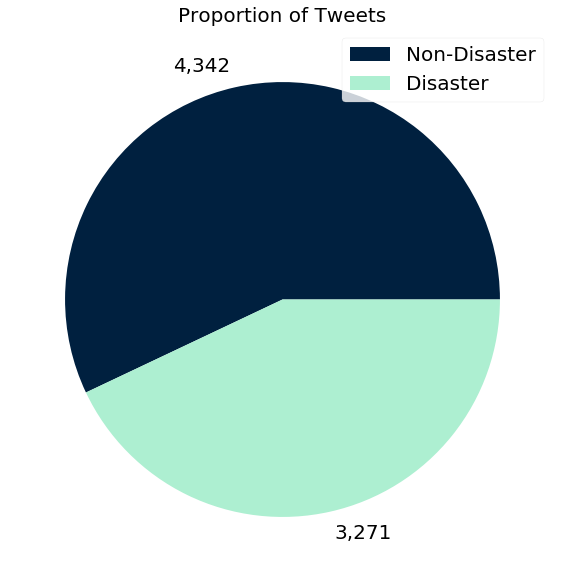
\includegraphics[width=0.7\linewidth]{../figures/class_proportion.png}
  \caption{Class proportions.}
  \label{fig:class_proportions}
\end{figure}

\section{Quantitative Statistics}
% # tokens, word frequencies, emojis, # words/tweet, URLs, POS, punctuation,
% spellcorrections
Exploring the textual data in the corpus reveals some correlations between the
various syntactic and semantic features, and the two classes. Figure
\ref{fig:num_words} shows that there is a small shift in the mean of the
average number of words per tweet between the two classes. Non-disaster (fake)
tweets are, on average, shorter and have a larger variation in tweet size. This
implies that the tweet length could be a useful feature for classification.\\

\begin{figure}[hbt!]
  \centering
  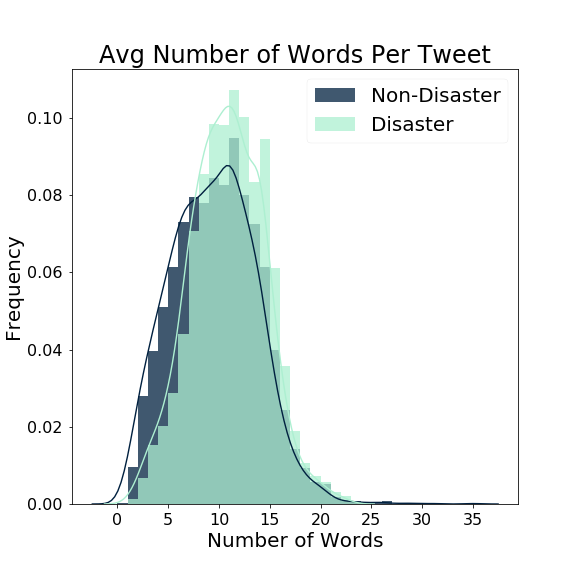
\includegraphics[width=0.7\linewidth]{../figures/num_words.png}
  \caption{Distribution of average number of words per tweet.}
  \label{fig:num_words}
\end{figure}

Emojis have a prominent presence in social media, also on Twitter.
Unfortunately, the text in the dataset is encoded in such a way that emojis can
not be distinguished from each other. However, one can still look at the
frequency of their use. \textit{A priori} one could argue that a real disaster tweet
is often from a mainstream news source and would stray away from using informal
language and symbols, such as emojis. Figure \ref{fig:emoji_freq}, showing the
frequency of emoji-usage, confirms this hypothesis. Non-disaster tweets use
emojis more regularly than real disaster tweets. Since emojis are encoded as a
special escape-sequence they can be considered as a semantic token equivalently
to a regular word when modeling the problem for classification.

\begin{figure}[hbt!]
  \centering
  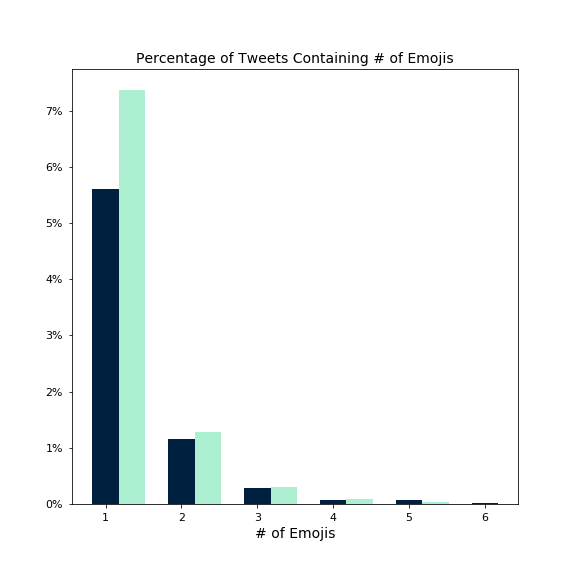
\includegraphics[width=0.7\linewidth]{../figures/emoji_freq.png}
  \caption{Frequency of emoji-usage in the two classes.}
  \label{fig:emoji_freq}
\end{figure}

The use of external links has shown to be a large differentiator between the
two classes. 50\% of non-disaster tweets contain external links, compared to
78\% of disaster tweets. A rationale for this difference is that disaster
tweets often refer to a source or proof of the disaster. Looking into the links
being used, we can observe a difference in pages that are linked to from the
two classes. Figure \ref{fig:domain_freq} shows the top 15 referred-to domains
by the two classes. Observe that the disaster tweets are linking to official
news sites such as \texttt{bbc.co.uk}, \texttt{latimes.com}, \texttt{cnn.com},
while the non-disaster tweets link to other social-medias sites such as
\texttt{facebook.com} and \texttt{instagram.com}, \texttt{ebay.com} and various
blogs. 

\begin{figure}[hbt!]
  \centering
  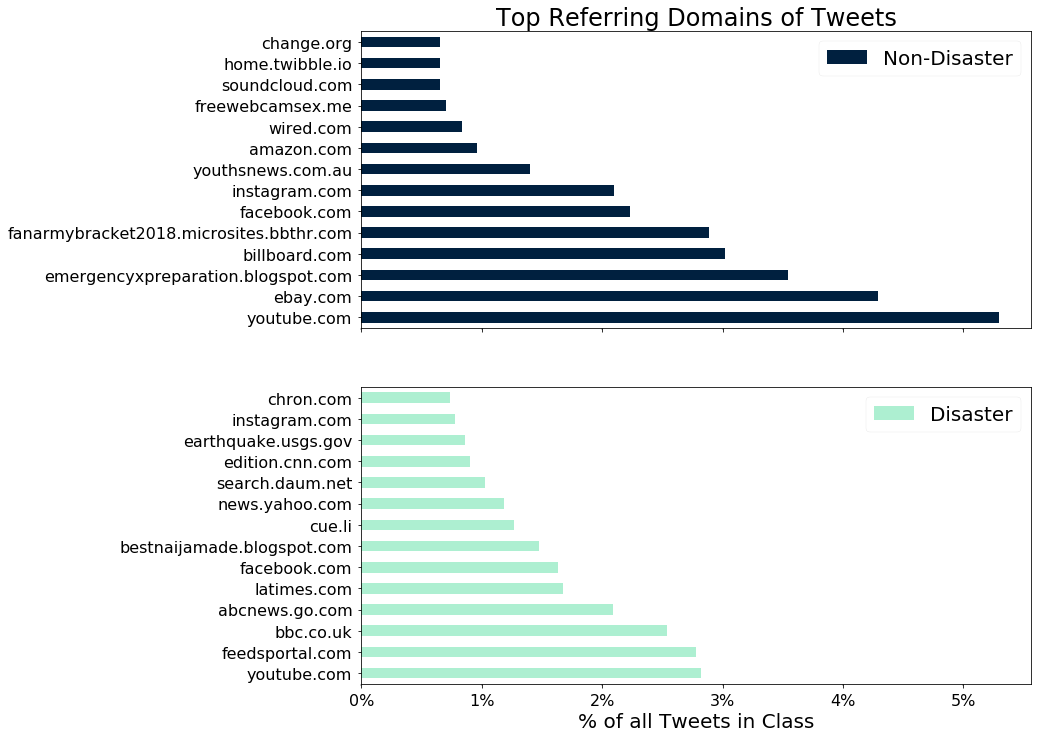
\includegraphics[width=\linewidth]{../figures/domain_freq.png}
  \caption{Top domains for links in tweets.}
  \label{fig:domain_freq}
\end{figure}

Punctuation ...
\begin{figure}[hbt!]
  \centering
  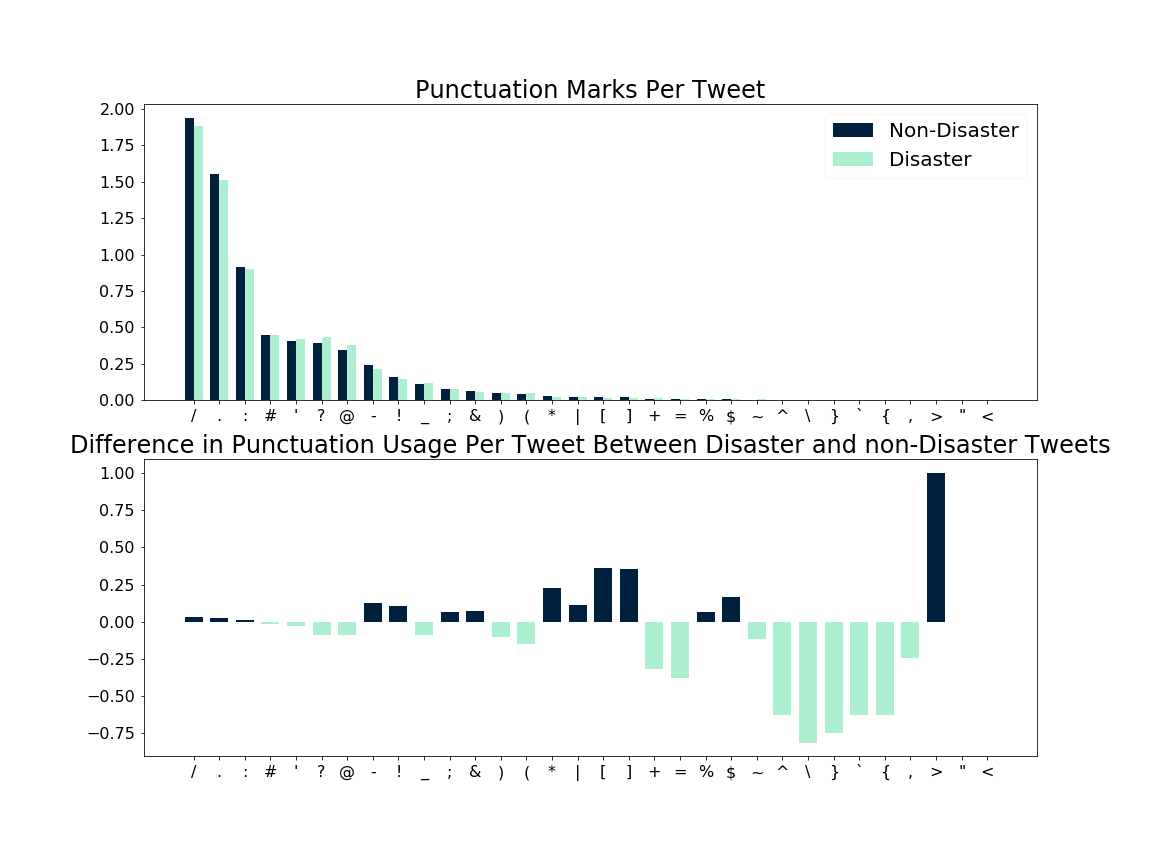
\includegraphics[width=\linewidth]{../figures/punctuation.png}
  \caption{Use of punctuation per tweet and differences in use between classes.}
  \label{fig:punctuation}
\end{figure}

Figure \ref{fig:part_of_speech} illustrates some of the different linguistic
feautres of the two classes by showing the distribution and difference in
part-of-speech tags per tweet. Notably, the disaster tweets more often use
numbers and proper nouns. One explaination of this difference would be the
larger amount of references to statistics (numbers) and official bodies and
names (proper nouns) in real disaster coverage. However, the difference is very
minimal for all POS-tags, so this could simply be an arbitrary difference due
to noise. The \texttt{en\_core\_web\_sm} POS-tagger in \texttt{spacy} was used for
tagging.

\begin{figure}[hbt!]
  \centering
  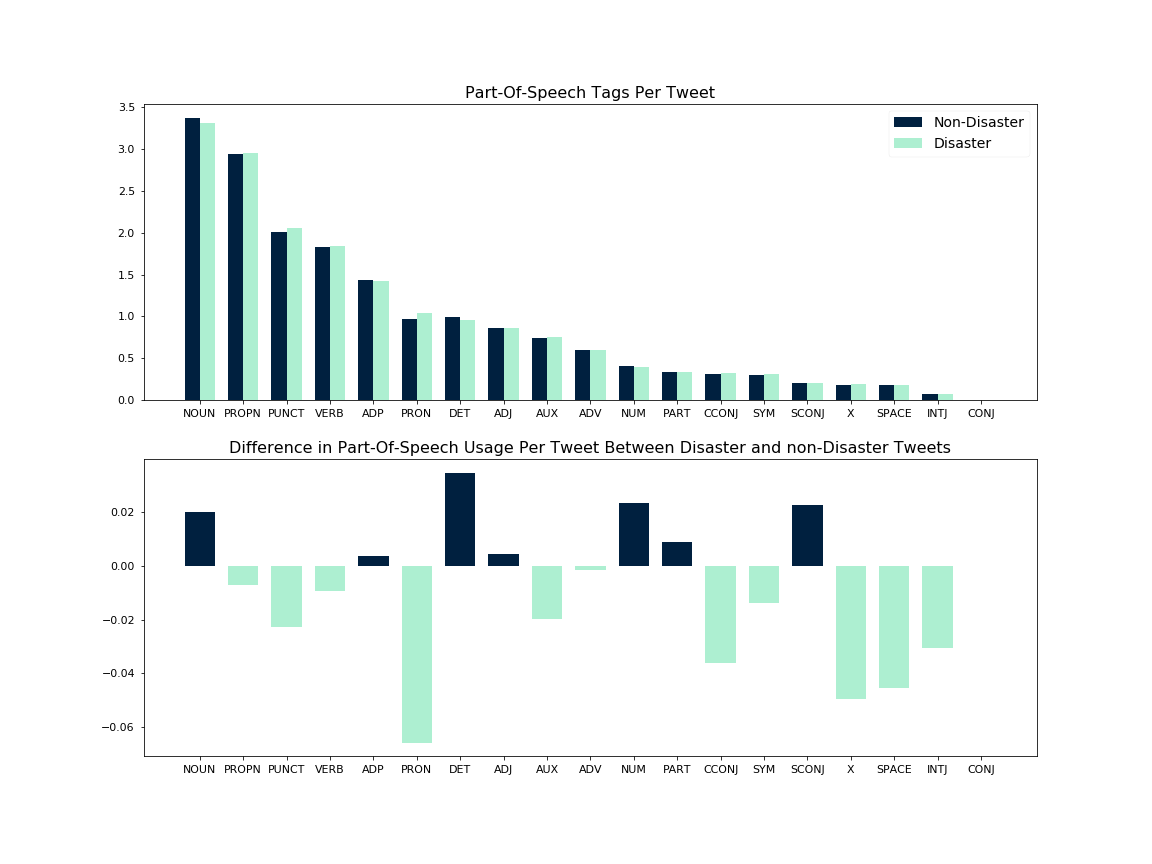
\includegraphics[width=\linewidth]{../figures/part_of_speech.png}
  \caption{Distribution of POS tags per tweet and differences between classes.}
  \label{fig:part_of_speech}
\end{figure}

Using a Hamilton distance of 1 between two tokens and the WordFrequency
project\footnote{https://github.com/hermitdave/FrequencyWords} dictionary to
correct spelling, we evaluate the number of spelling mistakes per tweet, per
class. Figure \ref{fig:spelling_mistakes} shows the number of spelling
mistakes for both classes. We observe that except for tweets with a single
spelling mistake, disaster tweets contain more mistakes than non-disaster
tweets. These differences are very small and lay within the margin of error to
be expected from approach to detecting spelling mistakes used. 

\begin{figure}[hbt!]
  \centering
  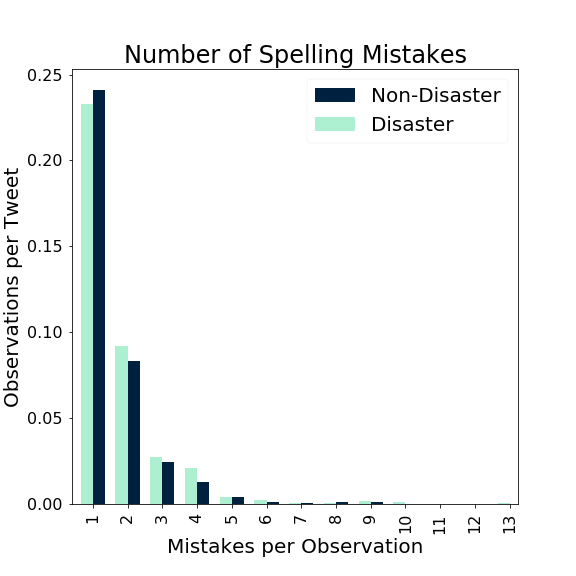
\includegraphics[width=0.9\linewidth]{../figures/spelling_mistakes.png}
  \caption{Frequency of spelling mistakes per tweet.}
  \label{fig:spelling_mistakes}
\end{figure}

\section{Sentiment analysis}
As we have seen from the investigation into the use of external links, many of
the real disaster tweets are referring to large mainstream news sources. News
is supposed to be objective and carry little to no sentiment. Using VADER
Sentiment Analysis\footnote{\url{https://github.com/cjhutto/vaderSentiment}}, a
rule-based sentiment analysis tool that is specifically made for social media
text, we investigate the correlation between sentiment and subjectivity, and
classes. Figure \ref{fig:sent_sub_dist} shows a distribution and density of
sentiment and subjectivity scores. Note that the two classes are laid on top of
each other in both figures. A negative sentiment value naturally corresponds to
negative sentiment, positive values correspond to positive sentiment and 0
corresponds to a neutral or non-sentimental tweet. A subjectivity score of 0
corresponds to an objective text, where 1 corresponds to maximum subjectivity.

\begin{figure}[hbt!]
  \centering
  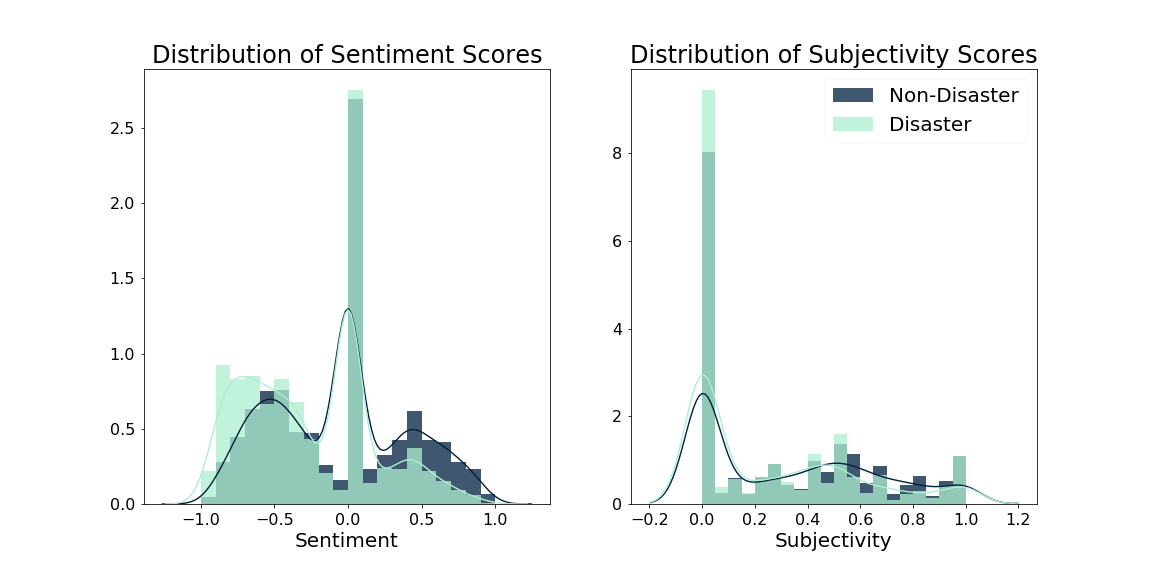
\includegraphics[width=\linewidth]{../figures/sent_sub_dist.png}
  \caption{Distribution and sentiment }
  \label{fig:sent_sub_dist}
\end{figure}

Observe that disaster tweets are more frequently objective and neutral.
Additionally, non-disaster tweets carry more positive sentiment while disaster
tweets are negative more often. Non-disaster tweets are also slightly skewed
towards being more subjective than real disaster tweets. These observations all
follow the intuition of disaster tweets being either mostly neutral and
objective (reported news) or carry a negative sentiment. 

\begin{table}[hbt!]
  \begin{center}
   \begin{tabular}{c|c|c|c|c} 
   \hline
    \textbf{Class} & \textbf{Negative} & \textbf{Neutral} & \textbf{Positive} & \textbf{Subjective}\\
    Non-Disaster & 0.132 & 0.766 & 0.102 & 0.324\\
    Disaster & 0.173 & 0.777 & 0.049 & 0.265\\
   \hline
  \end{tabular}
  \end{center}
  \caption{Mean values of negative, neutral and positive sentiment as well as
  mean subjectivity of tweets for each class.}
  \label{tab:sentiment}
\end{table}

Table \ref{tab:sentiment} shows the mean values of sentiment and
subjectivity for the two classes. These values further quantifies the
differences. Disaster tweets are 20\% more objective, 71\% less positive
and 27\% more negative than non-disaster tweets. 

\section{Feature Exploration}
% TF-IDF + cosine, D-tree vis, PCA, n-grams. Non-ML modeling,

\section{Conclusion}

% Can use something like this to put references on a page
% by themselves when using endfloat and the captionsoff option.
\ifCLASSOPTIONcaptionsoff
  \newpage
\fi

% trigger a \newpage just before the given reference
% number - used to balance the columns on the last page
% adjust value as needed - may need to be readjusted if
% the document is modified later
%\IEEEtriggeratref{8}
% The "triggered" command can be changed if desired:
%\IEEEtriggercmd{\enlargethispage{-5in}}

% references section

% can use a bibliography generated by BibTeX as a .bbl file
% BibTeX documentation can be easily obtained at:
% http://www.ctan.org/tex-archive/biblio/bibtex/contrib/doc/
% The IEEEtran BibTeX style support page is at:
% http://www.michaelshell.org/tex/ieeetran/bibtex/
\bibliographystyle{IEEEtran}
% argument is your BibTeX string definitions and bibliography database(s)
%\bibliography{IEEEabrv,../bib/paper}
%
% <OR> manually copy in the resultant .bbl file
% set second argument of \begin to the number of references
% (used to reserve space for the reference number labels box)

\bibliography{references.bib}

\end{document}
